\documentclass[sigconf]{acmart}

\usepackage{graphicx}
\usepackage{hyperref}
\usepackage{todonotes}

\usepackage{endfloat}
\renewcommand{\efloatseparator}{\mbox{}} % no new page between figures

\usepackage{booktabs} % For formal tables

\settopmatter{printacmref=false} % Removes citation information below abstract
\renewcommand\footnotetextcopyrightpermission[1]{} % removes footnote with conference information in first column
\pagestyle{plain} % removes running headers

\newcommand{\TODO}[1]{\todo[inline]{#1}}

\begin{document}
\title{Big Data Analytics on Food Products Around the World}

\author{Karthik Vegi}
\affiliation{%
  \institution{Indiana University Bloomington}
  \streetaddress{College Mall Apartments}
  \city{Bloomington} 
  \state{Indiana} 
  \postcode{47401}
  }
\email{kvegi@iu.com}

\author{Nisha Chandwani}
\orcid{1234-5678-9012}
\affiliation{%
  \institution{Indiana University Bloomington}
  \streetaddress{Park Doral Apartments}
  \city{Bloomington} 
  \state{Indiana} 
  \postcode{47405}
}
\email{nchandwa@iu.edu}

% The default list of authors is too long for headers}
\renewcommand{\shortauthors}{kvegi,nchandwa}

\begin{abstract}
Food is one of the basic necessities of human-being. It helps us gain energy to recharge our body to do the daily activities like moving, playing, and thinking. From being a cave man to producing wide variety of foods, we have come a long way. The civilizations shaped the food habits of the world and there is a lot of variance in the food habits across countries. We analyze the {\em Open Food Facts} database that gathers information on food products from around the world to unearth some food habits of the world and we predict the food grade based on the nutrition facts of the food products.
\end{abstract}

\keywords{i523, hid231, hid203, big data, food habits, food products, nutrition}

\maketitle

\section{Introduction}
{\em Open Food Facts} is a non-profit initiative started by Stephane Gigandet and run by thousands of volunteers around the world. Any person around the world can contribute to the database by simply scanning a product using a mobile app which is made available to IOS and Android. This massive database of food products opens up a lot of opportunities to analyze the food products around the world and understand their food habits. We are particularly interested in the consumption of good nutrients and some bad nutrients.

\section{Nutrition Grade Labelling System}
France recently took a decision to implement a nutri-score system which will use a color coding mechanism to label the food products that will help consumers know the nutrition grade of the product \cite{www-who}. The World Health Organization regional office for Europe as a part of its 5 year action plan from 2015-2020 recommends a labelling mechanism for the consumers to know about the quality of the food products at a first glance \cite{www-who}. This will not only make it easier for the consumers to pick healthier options but it will also regulate food manufacturers to resort to healthier ingredients instead of going for low cost artificial or less healthier ingredients \cite{www-who}.  \\

France after United Kingdom became the second country to implement this system to indicate the main ingredients like fat, salt and sugar content in the food items \cite{www-who}. France made use of an evidence based system to study different labelling systems to arrive at the best one \cite{www-who}. By implementing this system, the World Health Organization will keep a check on the growing number of diet related diseases in the Europe region \cite{www-who}. Europe being the largest consumer of cheese wants to regulate the ingredients that go into the manufacturing process so that people are well informed about their food choices \cite{www-who}.

\subsection{Nutrition Grade Prediction as a Big Data Problem}
We build a predictive classification model to predict the food nutrition grade based on the ingredients of the food. The goal is to apply various machine learning algorithms to the problem at hand, measure the prediction accuracy to compare and contrast the different algorithms, and arrive at the best algorithm that suits the given data and the problem. This problem can be solved using Big Data and Machine Learning techniques given the size and the complexity of the data.

\section{Machine Learning}
Machine Learning is a field in which we train computers in a way that they can learn from the input data \cite{book-shai}. The ideology is that computers use the training data that is made available to them, learn from it, build a model and use this experience to build knowledge that can be applied on new unseen data \cite{book-shai}. A wonderful example to demonstrate machine learning is the application to detect spam emails where the machine builds knowledge from previously seen emails which are marked as spam, checks new emails to see if they match the historic spam emails and label them as spam or non-spam \cite{book-shai}. 

\subsection{Types of Machine Learning Algorithms}
There are primarily two types of machine learning algorithms which are descriptive models and predictive models \cite{book-shai}. A {\em Descriptive Model} is described as the analysis done and insights gained from slicing and dicing the data in new and interesting ways \cite{book-shai}. One example of descriptive model is patter discovery that is often used in market basket analysis where transnational purchase details are analyzed \cite{book-shai}. A {\em Predictive Model} on the other hand involves predicting one value using one or more variables \cite{book-shai}. The learning algorithms tried to build a model that captures the relationship between a response variables and dependent target variables \cite{book-tan}.

\subsection{Types of Learning}
{\em Unsupervised Learning} is the process where there is no explicit training data to learn from, so there is simply no mechanism where the machine can learn from previously available data \cite{book-shai}. The same email example can be looked at in a different way where we now want to do anomaly detection in emails \cite{book-shai}. Here the main goal is to detect unusual messages from the bunch of messages and we do not have experience of previous data \cite{book-shai}. \\

{\em Supervised Learning} in contrast is the process of gaining knowledge or expertise from the training data which can be applied to future unseen data \cite{book-shai}. Here the model is first trained by using a bulk of training examples and this model is applied against testing data to measure the accuracy \cite{book-shai}. The variable that we need to predict is identified which is called the response variable and the variables that are used to predict the response variables, called the predictor variables are identified \cite{book-shai}. If the existing variables are not sufficiently giving the accuracy that is expected, a method called feature engineering is done where new variables are derived by combining existing variables \cite{book-shai}. 

\section{Prediction Analysis}
Prediction analysis is the process of working on  a large data set using a combination of statistical, data mining and machine learning algorithms to predict the outcome based on past data \cite{book-shai}.
There are primarily two types of prediction analysis in machine learning, namely regression and classification \cite{book-tan}. In regression, we try to predict a continuous variable from the predictor variables \cite{book-tan}. A good example of regression is to predict the housing prices from different parameters like year of construction, location, amenities, number of bed rooms etc \cite{book-tan}. Here the response variable is continuous and it is not predefined \cite{book-tan}. Classification on the other hand tries to predict a categorical variable in which we assign each record with a predefined label or a class \cite{book-tan}. \\

Classification is the task of assigning each data record to a predefined class \cite{book-tan}. In machine learning, classification is categorized as a supervised learning technique \cite{book-tan}. This problem has applications in various fields like spam detection, medical applications, astronomy and banking to identify fraudulent transactions from genuine transactions \cite{book-tan}. It is the task as coming up with a model which is essentially a function that maps every data record to a class label \cite{book-tan}. \\ 

The task at hand is a classification problem since we are trying to predict the food nutrition grade of the products based on the ingredients that go into the product. For this problem we are considering only the data for the country France, since the nutrition grade is available for most food products from the country. Another reason is that France is the first countries in the region to come up with the idea of adding a color coded label to the food products mentioning the nutrition grade. In the subsequent sections we discuss the machine learning techniques used to solve this problem.

\subsection{K Nearest Neighbors}

\subsubsection{Overview} Some of the classification algorithms in machine learning work on the principle of eager learning that involves a two step process where first a model is built from the training data and the model is applied on testing data \cite{book-tan}. In contrast, K nearest neighbors is a lazy learning algorithm where the process of modeling the training data is not done until the test examples are classified \cite{book-tan}. {\em Rote Classifier} is a good example of lazy learning algorithm memorizes the entire training data to perform classification but has the drawback of not being able to map every test example against the training example \cite{book-tan}. K nearest neighbors algorithm overcomes this drawback by finding all the records that are closest or nearest to the training records \cite{book-tan}. \\

The nearest neighbour puts each attribute list as a data point in the n-dimensional space, given n the number of attributes \cite{book-tan}. Once we have the training examples, we take each test example and compute its distance to the training example classes and assign a class label \cite{book-tan}. Any of the popular distance measures among Euclidean distance, Manhattan distance, Minkowski distance and Mahalanobis distance can be used \cite{book-tan}. The k denotes the k closest points to the test example \cite{book-tan}. Figure \ref{fig:Fig1} shows the structure of the data \cite{book-tan}.

\begin{figure}
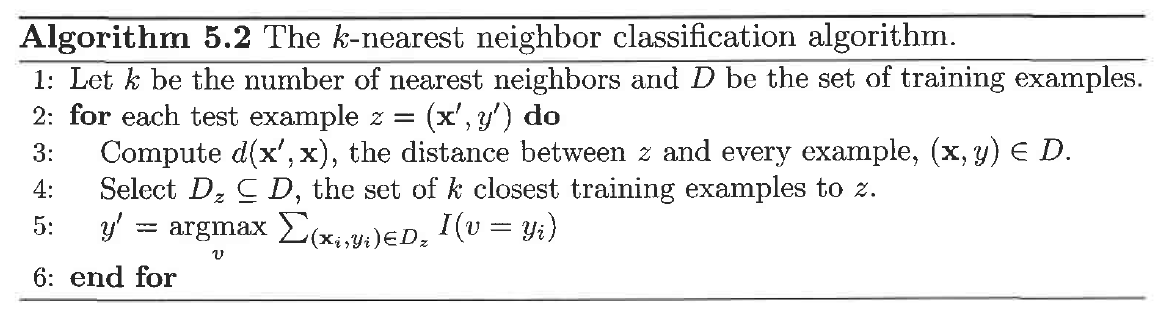
\includegraphics[width=1.0\textwidth]{images/fig1.png}
\caption{K nearest neighbors algorithm\cite{book-tan}}
\label{fig:Fig1}
\end{figure}

\subsubsection{Support in Python} 
KNeighborsClassifier is available in the scikit learn python library. 

\subsection{Logistic Regression}
Logistic regression or logit regression is a special type of regression analysis where the response variable that we need to predict is a categorical variable \cite{book-tan}. Typically logistic regression models the response variable to take two values 1 or 0, pass or fail, win or lose \cite{book-tan}. Logistic regression that takes more than two values for the response variable is called multinomial logistic regression \cite{book-tan}. Here the probability of the response variable to take a categorical value is modelled as a function of the predictor variables \cite{book-tan}. \\

Like a lot of machine learning algorithms, logistic regression works by making a lot of assumptions which should be taken care as a part of the data cleaning and transformation process \cite{book-shai}. It does not assume a linear relationship between the response variables and predictor variables \cite{book-shai}. Since it applies a log transformation on the predicted probabilities, it can handle a variety of relationship between the predictor variables \cite{book-shai}. If the predictor variables are multivariate normal, the algorithm achieves best result although it works even if they are not \cite{book-shai}. Stepwise method must be used in the logistic regression to ensure that we are neither overfitting nor underfitting the data \cite{book-shai}. A very important assumption to be noted in logistic regression is that the each attribute list must be independent, in the sense the data records must not be derived from a before-after setup experiment \cite{book-shai}. It also requires a decently large sample size to work on \cite{book-shai}. 

\subsubsection{Support for Python} LogisticRegression is available in the scikit learn python library.

\subsection{Random Forest Classifier}
Random forest is a ensemble classification algorithm which is very powerful \cite{book-tan}. Ensemble method is a special process to improve the accuracy of the prediction \cite{book-tan}. The classification algorithms we have seen so far predict the response variable using a single classifier on the test data but ensemble methods use multiple classfiers in tandem and aggregate the predictions to boost the accuracy by a huge margin \cite{book-tan}. Using a combination method, the ensemble method derives a set of base classifiers from the training data and on each iteration takes a vote of all the base classifiers to arrive at a result \cite{book-tan}. \\

Random forest is an ensemble method which works very well for classification problems \cite{book-tan}. It combines the predictions made by multiple classifiers where each classifier independently works on the training data and casts its vote \cite{book-tan}. Unlike methods like AdaBoost which generates values based on independent random vectors using a varied probability distribution, random forest generates values based on fixed probability distribution \cite{book-tan}. 

\subsubsection{Rationale for Random Forest}
Consider an example, where we have 25 base classifiers and each base classifier has an error rate of 0.35 \cite{book-tan}. As discussed, the random forest takes the majority vote given by the base classifiers \cite{book-tan}. The model makes a wrong prediction if half or more base classifiers predict wrong, if not the accuracy is improved with an error rate of 0.06 which is far better than using just a single classifier \cite{book-tan}.

\subsubsection{Support for Python} RandomForestClassifier is available in the scikit learn python library.

\subsection {Algorithm and Methodology}

\subsection{Python Packages Used}
The following Python packages were used to solve the classification problem: \\
{\em Pandas} \\
{\em Matplotlib} \\
{\em Seaborn} \\
{\em Scikit-learn} \\
{\em Scipy} \\

\subsection{Data}
Number of examples: 123,961 \\
Number of variables: 12 \\
Response variables: {\em Nutrition Grade} \\
Predictor variables: {\em Energy per 100g, Fat per 100g, Saturated Fat per 100g, Carbohydrates per 100g, Sugars per 100g, Fiber per 100g, Proteins per 100g, Salt per 100g, Trans-fat per 100g, Sodium per 100g}

\subsection{Data Cleaning and Transformation}
Step 1: \\
We first check the data value counts for each country. United States, France, Switzerland, Germany and Spain come as the top 5 countries with most data. Since the food nutrition grade was implemented in France, it has most products with the data available so for this classification problem we use the data filtered on France. 

Step 2: \\ Cleaning
Handling missing values
- why is it a problem
- missing, missing at random
- imputation: mean, mode,
we got better results by dropping missing values
Outlier treatment

Step 3: \\ Transformation
- why standardization of data is important (skewness)
massive improvement in results after standardization
random forest for missing values
scaling
standard scaler

Step 4: EDA \\
box plots, inference from box plots
correlation - multi-collinearity, 
handling multi-collinearity - feature engineering,
remove sodium


\subsection{Sampling, Stratified sampling} 
one


Step 5: \\
\begin{itemize}
	\item Transformation: Join, filter, union, map and various other operations that can be performed on existing RDDs which result in a new RDD at the end of the operation, are referred to as transformations.
	\item Action: Count, first, reduce and various other operations which evaluate an existing RDD and return values at the end of these operations are referred to as Actions.
\end{itemize}

\section{Conclusion}


\begin{acks}

The author would like to thank Dr. Gregor von Laszewski and the teaching assistants for their support and suggestions.

\end{acks}

\bibliographystyle{ACM-Reference-Format}
\bibliography{report} 

\end{document}
